% Figure clh_lean_hessian: the Hessian form on a plane of the gauge directions, and Psi_f below its chord.
% Illustrates CLH-3 (Proposition prop:psd). Inputs: f-bar = (3,5,1,2,4), theta/pi = (0, 0.1, 0.7, 0.3, 0.8), h = x e_3 + y e_2 (so h_1 = 0), segment from theta to theta + 0.02 pi e_3.
% Source of the figure, typeset in the paper's own fonts (T1, Latin Modern, 11pt) at the paper's text
% width (6.5in), so \includegraphics does not rescale it. It adds no assertion.
% Every coordinate is read from numerical values computed by floating-point code that follows the
% paper's formulas (the pictures' Lean helper); the SHA-256 of each output line it comes from:
%   D50_s53_default 64e2a49cc7ed0b894e4b8c439c68e37a5fa379eaa234dbfe255eb967871fa5ef
%   D52_s54_default 3d4c06e47f1c3fc7d4327da3963615060db762acdab9def3d4d5b59cc9dea252
% Build: pdflatex <this file> && pdftocairo -svg <this file>.pdf <this file>.svg

\documentclass[11pt]{standalone}
\usepackage[T1]{fontenc}
\usepackage{lmodern}
\usepackage{amsmath,amssymb}
\usepackage{tikz}
\usetikzlibrary{arrows.meta,calc}

% the palette of the paper's other figures: blue solid for the first object, ochre dashed for the second
\definecolor{ink}{HTML}{233740}
\definecolor{muted}{HTML}{65757D}
\definecolor{pblue}{HTML}{0072B2}
\definecolor{qochre}{HTML}{B87827}

\tikzset{
  ax/.style={draw=muted, line width=0.5pt},
  axd/.style={draw=muted!70, line width=0.4pt, dash pattern=on 1.5pt off 2pt},
  tick/.style={draw=muted, line width=0.5pt},
  lab/.style={font=\footnotesize, inner sep=1.2pt, text=ink},
  labm/.style={font=\small, inner sep=1.2pt, text=ink},
  labw/.style={font=\footnotesize, inner sep=1pt, text=ink, fill=white, fill opacity=0.8, text opacity=1},
  labP/.style={font=\footnotesize, inner sep=1.2pt, text=pblue},
  labQ/.style={font=\footnotesize, inner sep=1.2pt, text=qochre},
  tk/.style={font=\footnotesize, inner sep=1pt, text=muted},
  panel/.style={font=\small, inner sep=0pt, text=ink},
  curveP/.style={pblue, line width=1.1pt, line cap=round, line join=round},
  thinP/.style={pblue, line width=0.8pt, line cap=round, line join=round},
  thinQ/.style={qochre, line width=0.8pt, dash pattern=on 3pt off 1.6pt, line cap=round, line join=round},
  curveQ/.style={qochre, line width=1.1pt, dash pattern=on 4pt off 1.6pt, line cap=round},
  fillP/.style={pblue, fill=pblue!8, line width=1.1pt, line join=round},
  dotI/.style={circle, draw=ink, fill=ink, line width=0.6pt, inner sep=0pt, minimum size=4.6pt},
  dotIs/.style={circle, draw=ink, fill=ink, line width=0.5pt, inner sep=0pt, minimum size=3.2pt},
  ringI/.style={circle, draw=ink, fill=white, line width=0.6pt, inner sep=0pt, minimum size=4.6pt},
  dotP/.style={circle, draw=pblue, fill=pblue, line width=0.6pt, inner sep=0pt, minimum size=4.6pt},
  dotQ/.style={circle, draw=qochre, fill=qochre, line width=0.6pt, inner sep=0pt, minimum size=4.6pt},
  dotQs/.style={circle, draw=qochre, fill=qochre, line width=0.5pt, inner sep=0pt, minimum size=3pt},
  ringQ/.style={circle, draw=qochre, fill=white, line width=0.6pt, inner sep=0pt, minimum size=4.6pt},
}

\begin{document}
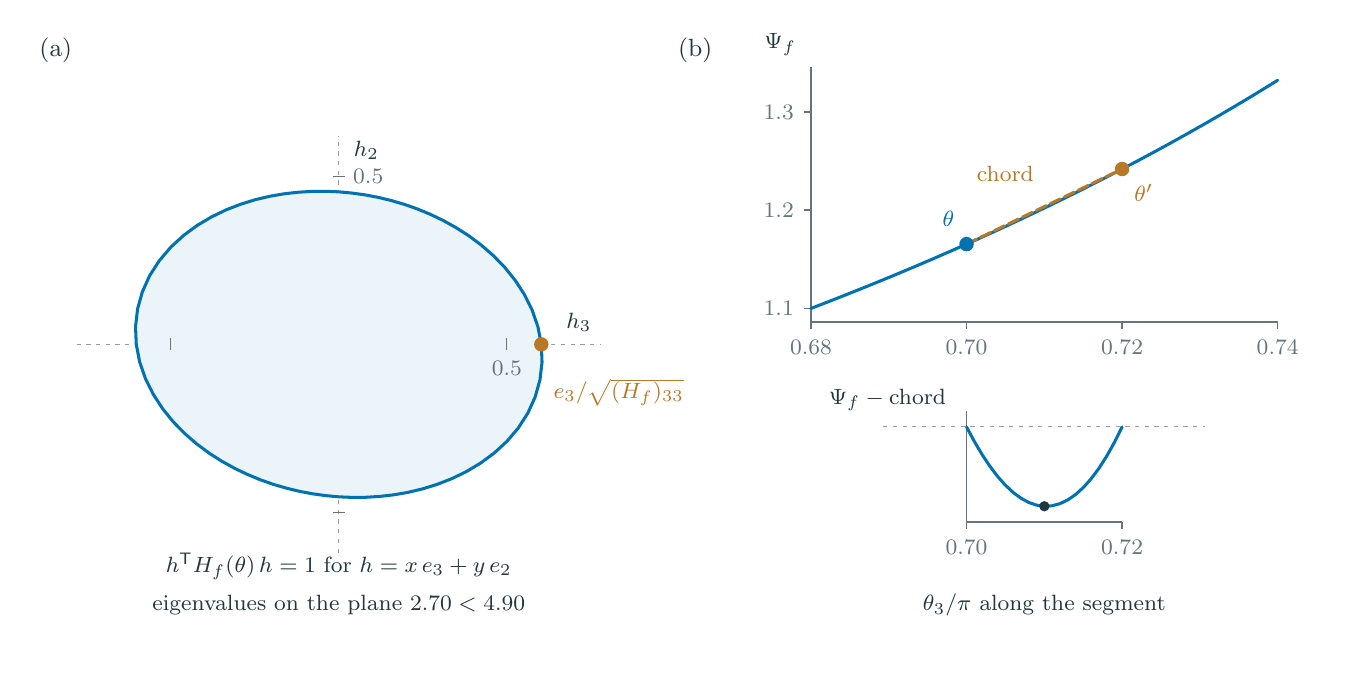
\begin{tikzpicture}[x=1bp,y=1bp]
\useasboundingbox (0bp,0bp) rectangle (468bp,224bp);
%box A 17.64516129 35 188.7096774 150 -0.78 0.78 -0.62 0.62
\draw[axd] (17.65,110.00) -- (206.35,110.00); %line
\draw[axd] (112.00,35.00) -- (112.00,185.00); %line
\draw[fillP] (184.91,110.00) -- (183.70,116.27) -- (181.63,122.28) -- (178.84,127.91) -- (175.47,133.10) -- (171.66,137.82) -- (167.52,142.06) -- (163.17,145.83) -- (158.68,149.17) -- (154.09,152.09) -- (149.47,154.65) -- (144.82,156.87) -- (140.17,158.79) -- (135.51,160.42) -- (130.85,161.78) -- (126.18,162.91) -- (121.49,163.80) -- (116.76,164.46) -- (112.00,164.90) -- (107.18,165.10) -- (102.29,165.06) -- (97.33,164.76) -- (92.28,164.19) -- (87.15,163.30) -- (81.94,162.07) -- (76.68,160.45) -- (71.39,158.39) -- (66.14,155.86) -- (61.00,152.79) -- (56.07,149.16) -- (51.49,144.94) -- (47.39,140.13) -- (43.94,134.77) -- (41.30,128.94) -- (39.57,122.77) -- (38.83,116.40) -- (39.09,110.00) -- (40.30,103.73) -- (42.37,97.72) -- (45.16,92.09) -- (48.53,86.90) -- (52.34,82.18) -- (56.48,77.94) -- (60.83,74.17) -- (65.32,70.83) -- (69.91,67.91) -- (74.53,65.35) -- (79.18,63.13) -- (83.83,61.21) -- (88.49,59.58) -- (93.15,58.22) -- (97.82,57.09) -- (102.51,56.20) -- (107.24,55.54) -- (112.00,55.10) -- (116.82,54.90) -- (121.71,54.94) -- (126.67,55.24) -- (131.72,55.81) -- (136.85,56.70) -- (142.06,57.93) -- (147.32,59.55) -- (152.61,61.61) -- (157.86,64.14) -- (163.00,67.21) -- (167.93,70.84) -- (172.51,75.06) -- (176.61,79.87) -- (180.06,85.23) -- (182.70,91.06) -- (184.43,97.23) -- (185.17,103.60) -- (184.91,110.00) -- cycle; %poly A/ellipse
\draw[tick] (51.52,107.80) -- (51.52,112.20); %tickx A -0.5
\draw[tick] (109.80,49.52) -- (114.20,49.52); %ticky A -0.5
\draw[tick] (172.48,107.80) -- (172.48,112.20); %tickx A 0.5
\node[tk] at (172.48,101.50) {$0.5$}; %num A-xt 0.5
\draw[tick] (109.80,170.48) -- (114.20,170.48); %ticky A 0.5
\node[tk, anchor=west] at (116.00,170.48) {$0.5$}; %num A-yt 0.5
\node[dotQ] at (184.91,110.00) {}; %dot A/u1
\node[labQ, anchor=north west] at (187.91,99.00) {$e_3/\sqrt{(H_f)_{33}}$}; %t A-u1
\node[lab, anchor=east] at (204.35,118.00) {$h_3$}; %t A-h3
\node[lab, anchor=west] at (116.00,180.00) {$h_2$}; %t A-h2
\node[lab] at (112.00,30.00) {$h^{\mathsf T}H_f(\theta)\,h=1$ for $h=x\,e_3+y\,e_2$}; %t A-cap1
\node[lab] at (112.00,16.00) {eigenvalues on the plane $2.70<4.90$}; %num A-eig 2.70,4.90
\node[panel, anchor=west] at (4.00,216.00) {(a)}; %t A-tag
%box B 282 118 168 92 0.68 0.74 1.085897567 1.346336333
\draw[ax] (282.00,118.00) -- (450.00,118.00); %line
\draw[ax] (282.00,118.00) -- (282.00,210.00); %line
\draw[tick] (282.00,118.00) -- (282.00,115.50); %tickx B 0.68
\node[tk] at (282.00,109.00) {$0.68$}; %num B-xt 0.68
\draw[tick] (338.00,118.00) -- (338.00,115.50); %tickx B 0.7
\node[tk] at (338.00,109.00) {$0.70$}; %num B-xt 0.7
\draw[tick] (394.00,118.00) -- (394.00,115.50); %tickx B 0.72
\node[tk] at (394.00,109.00) {$0.72$}; %num B-xt 0.72
\draw[tick] (450.00,118.00) -- (450.00,115.50); %tickx B 0.74
\node[tk] at (450.00,109.00) {$0.74$}; %num B-xt 0.74
\draw[tick] (282.00,122.98) -- (279.50,122.98); %ticky B 1.1
\node[tk, anchor=east] at (277.00,122.98) {$1.1$}; %num B-yt 1.1
\draw[tick] (282.00,158.31) -- (279.50,158.31); %ticky B 1.2
\node[tk, anchor=east] at (277.00,158.31) {$1.2$}; %num B-yt 1.2
\draw[tick] (282.00,193.63) -- (279.50,193.63); %ticky B 1.3
\node[tk, anchor=east] at (277.00,193.63) {$1.3$}; %num B-yt 1.3
\draw[curveP] (282.00,122.93) -- (286.20,124.55) -- (290.40,126.19) -- (294.60,127.84) -- (298.80,129.52) -- (303.00,131.21) -- (307.20,132.92) -- (311.40,134.65) -- (315.60,136.40) -- (319.80,138.17) -- (324.00,139.96) -- (328.20,141.78) -- (332.40,143.61) -- (336.60,145.46) -- (340.80,147.34) -- (345.00,149.23) -- (349.20,151.15) -- (353.40,153.09) -- (357.60,155.06) -- (361.80,157.05) -- (366.00,159.06) -- (370.20,161.09) -- (374.40,163.15) -- (378.60,165.24) -- (382.80,167.35) -- (387.00,169.49) -- (391.20,171.65) -- (395.40,173.84) -- (399.60,176.06) -- (403.80,178.31) -- (408.00,180.58) -- (412.20,182.89) -- (416.40,185.22) -- (420.60,187.59) -- (424.80,189.98) -- (429.00,192.41) -- (433.20,194.88) -- (437.40,197.37) -- (441.60,199.90) -- (445.80,202.47) -- (450.00,205.07); %poly B/psi
\draw[curveQ] (338.00,146.08) -- (394.00,173.11); %poly B/chord
\node[dotP] at (338.00,146.08) {}; %dot B/theta
\node[dotQ] at (394.00,173.11) {}; %dot B/thetap
\node[labP, anchor=south east] at (335.00,151.08) {$\theta$}; %t B-theta
\node[labQ, anchor=north west] at (397.00,169.11) {$\theta'$}; %t B-thetap
\node[labQ, anchor=south east] at (363.60,167.06) {chord}; %t B-chordlab
\node[lab, anchor=east] at (278.00,218.00) {$\Psi_f$}; %t B-ylab
%box C 338 46 56 40 0.7 0.72 -0.001829376864 0.000304896144
\draw[ax] (338.00,46.00) -- (394.00,46.00); %line
\draw[ax] (338.00,46.00) -- (338.00,86.00); %line
\draw[tick] (338.00,46.00) -- (338.00,43.50); %tickx C 0.7
\node[tk] at (338.00,37.00) {$0.70$}; %num C-xt 0.7
\draw[tick] (394.00,46.00) -- (394.00,43.50); %tickx C 0.72
\node[tk] at (394.00,37.00) {$0.72$}; %num C-xt 0.72
\draw[axd] (308.00,80.29) -- (424.00,80.29); %line
\draw[curveP] (338.00,80.29) -- (340.80,75.04) -- (343.60,70.31) -- (346.40,66.11) -- (349.20,62.42) -- (352.00,59.27) -- (354.80,56.66) -- (357.60,54.59) -- (360.40,53.07) -- (363.20,52.11) -- (366.00,51.71) -- (368.80,51.89) -- (371.60,52.64) -- (374.40,53.97) -- (377.20,55.89) -- (380.00,58.42) -- (382.80,61.55) -- (385.60,65.29) -- (388.40,69.66) -- (391.20,74.65) -- (394.00,80.29); %poly C/gap
\node[dotIs] at (366.00,51.71) {}; %dot C/mid
\node[lab, anchor=east] at (332.00,90.00) {$\Psi_f-\text{chord}$}; %t C-ylab
\node[lab] at (366.00,16.00) {$\theta_3/\pi$ along the segment}; %t C-xlab
\node[panel, anchor=west] at (234.00,216.00) {(b)}; %t B-tag
\end{tikzpicture}
\end{document}
